%!TEX root = /Users/louis/Documents/PhD/Deliverables/Thesis/thesis.tex

\section{Evaluating User-Driven Co-Evolution}
\label{sec:exemplar_user-driven_co-evo}
User-driven co-evolution, a novel process for managing co-evolution, was identified in Chapter~\ref{Analysis}. In user-driven co-evolution, model migration is not specified in an executable form, and is instead performed by hand. This section first recaps Section~\ref{subsec:user-driven_co-evolution}, which describes the challenges to productivity faced by developers while performing user-driven co-evolution with EMF, arguably the most widely-used MDE development environment at present. Subsequently, two approaches to user-driven co-evolution are demonstrated and then compared. The first approach uses only those tools available in EMF; while the second approach uses EMF and, in addition, two of the structures presented in Chapter~\ref{Implementation}, a metamodel-independent syntax and a textual modelling notation. The section concludes by comparing the two approaches, highlighting that performing user-driven co-evolution using the structures proposed in Chapter~\ref{Implementation} mitigates some of the effects of the productivity challenges faces when performing user-driven co-evolution using only the tools available in EMF. Finally, ways in which this hypothesis might be evaluated more rigorously are discussed.


\subsection{Challenges for Performing User-Driven Co-Evolution}
Chapter~\ref{Analysis} highlighted two productivity challenges faced by developers while performing user-driven co-evolution in contemporary MDE environments. Firstly, model storage representations have not been optimised for use by humans, and hence user-driven co-evolution can be error-prone and time consuming. Secondly, the multi-pass parsers used to load models in contemporary MDE environments cause user-driven co-evolution to be an iterative process, because not all conformance errors are reported at once. The identification of these productivity challenges led to the derivation of the following research requirement: \emph{This thesis must demonstrate a user-driven co-evolution process that enables the editing of non-conformant models without directly manipulating the underlying storage representation and provides a conformance report for the original model and evolved metamodel.}

Two of the structures presented in Chapter~\ref{Implementation} provide the foundation for fulfilling the above research requirement. The first, a metamodel-independent syntax, facilitates the conformance checking of a model against any metamodel. The second structure, a textual modelling notation called HUTN, allows models to be managed in a format that is reputedly easier for humans to use than XMI, the canonical model storage format \cite{hutn}.

To fulfil the above research requirement, this section uses the metamodel-independent syntax and the textual modelling notation to demonstrate that user-driven co-evolution can be performed without encountering the challenges to productivity described above. To this end, an example of co-evolution is used to show the way in which user-driven co-evolution might be achieved with and without the metamodel-independent syntax and the textual modelling notation described in Chapter~\ref{Implementation}.

\subsection{Co-Evolution Example}
The remainder of this section uses a co-evolution example taken from collaborative work with Adam Sampson, then a Research Associate at the University of Kent. The purpose of the collaboration was to build a prototypical editor for graphical models of programs written in process-oriented programming languages, such as Occam-Pi\footnote{TODO: Check spelling, give citation}. The graphical models would provide a standard notation for describing process-oriented programs.

The graphical model editor was developed using MDE tools and techniques. A metamodel was used to capture the abstract syntax of process-oriented programming languages, and code for a graphical model editor was automatically generated from the metamodel. The final version of the graphical model editor is shown in Figure~\ref{fig:po_final_graphical_editor}.

\begin{figure}[htbp]
	\centering
	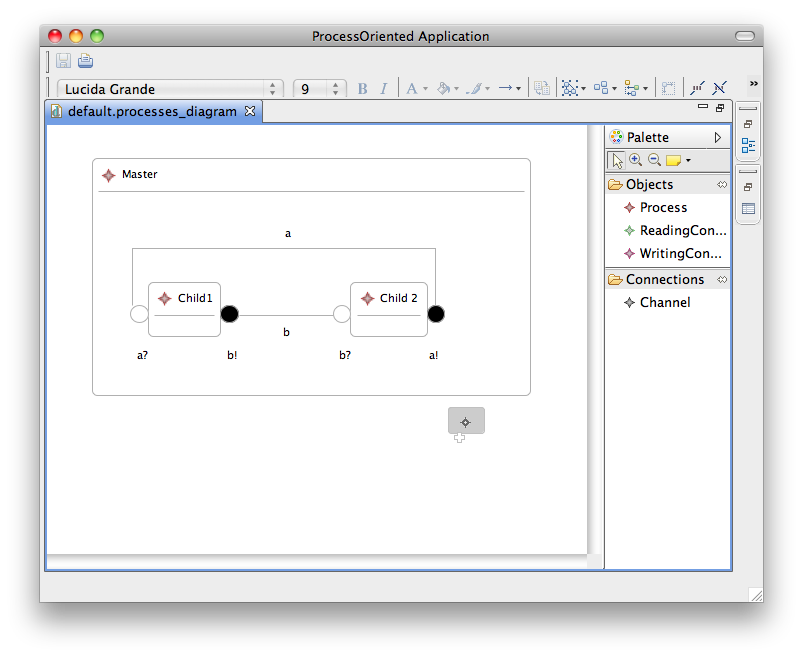
\includegraphics[width=13.5cm]{6.Evaluation/images/user_driven/po_final_editor.png}
	\caption{Final version of the prototypical graphical model editor.}
	\label{fig:po_final_graphical_editor}
\end{figure}


The editor was developed using the Eclipse Modeling Framework (EMF) \cite{steinberg09emf}, arguably the most widely-used contemporary MDE development environment. The metamodel was specified in Ecore, the metamodelling language of EMF, and a graphical model editor was generated from the metamodel using the Graphical Modeling Framework (GMF), an extension to EMF for graphical modelling. Section~\ref{sec:mde_tools} describes in more detail the way in which EMF and GMF can be used to specify metamodels and to generate graphical model editors.

The process-oriented metamodel was developed iteratively. During each iteration, the metamodel was changed. The remainder of this section uses an example of metamodel changes from one iteration of the project. The way in which development proceeded during that iteration is briefly described below.

\subsubsection{Feature identification}
The purpose of the iteration was to refine the representation of one of the domain concepts, \emph{connection points}. At the start of the iteration, the graphical model editor could be used to draw \emph{processes} (the fundamental building blocks of a process-oriented program), \emph{channels} (the mechanism by which processes communicate), and \emph{connection points} (which define the names and types of channel used by a process).

Figure~\ref{fig:po_original_editor} shows an exemplar model represented in the graphical model editor before the iteration began. The model contains two processes (depicted as boxes), \texttt{P1} and \texttt{P2}, one channel (depicted as a line), \texttt{a}, and two connection points (depicted as circles), \texttt{a!} and \texttt{a?}.

\begin{figure}[htbp]
	\centering
	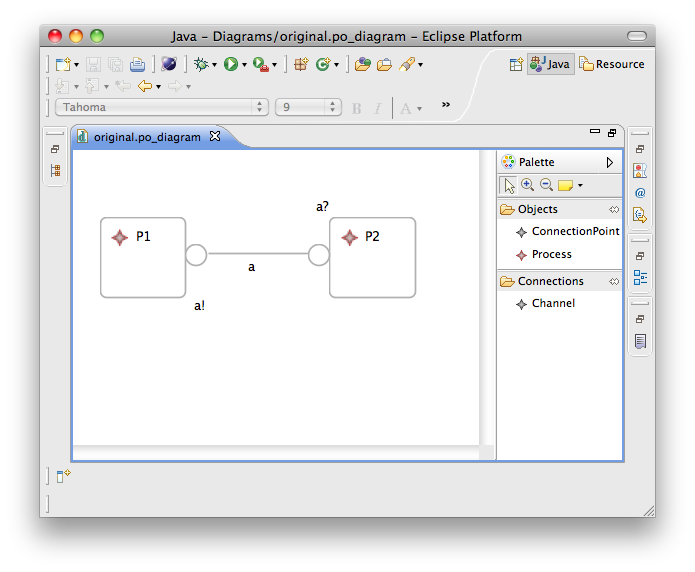
\includegraphics[width=13.5cm]{6.Evaluation/images/user_driven/po_original_editor.png}
	\caption{The graphical editor at the start of the iteration.}
	\label{fig:po_original_editor}
\end{figure}


The aim of the iteration was to distinguish between \emph{reading} and \emph{writing} connection points in the graphical notation. The former are used to receive messages, and the latter to send messages. In Figure~\ref{fig:po_original_editor}, \texttt{a?} and \texttt{b?} are intended to represent reading connection points, and \texttt{a!} a writing connection point. Sampson and the thesis author decided that the metamodel and graphical editor should be changed so that a shaded circle would be used represent writing connection points, and empty circles to represent reading connection points. At the end of the iteration the model shown in Figure~\ref{fig:po_original_editor} would be represented as shown in Figure~\ref{fig:po_evolved_editor}.

\begin{figure}[htbp]
	\centering
	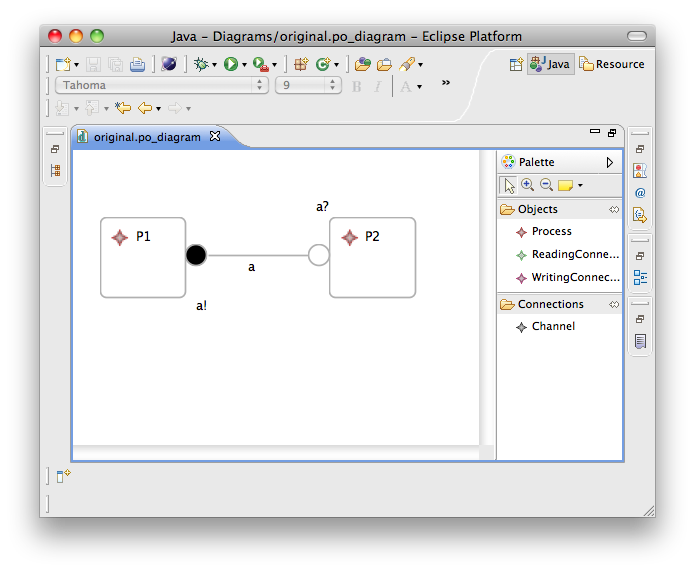
\includegraphics[width=13.5cm]{6.Evaluation/images/user_driven/po_evolved_editor.png}
	\caption{The graphical editor at the end of the iteration.}
	\label{fig:po_evolved_editor}
\end{figure}


\subsubsection{Implementation}
Before the iteration began, the metamodel did not distinguish between reading and writing \texttt{Co\-nn\-ec\-ti\-o\-nPo\-i\-nt}s. Figure~\ref{fig:po_original_mm} shows the way in which connection points were modelled at the start of the iteration. When a \texttt{Co\-nn\-ec\-ti\-o\-nPo\-i\-nt} was associated with a \texttt{Ch\-an\-nel}, the  \texttt{Co\-nn\-ec\-ti\-o\-nPo\-i\-nt} is specified as a \texttt{re\-ad\-er} or a \texttt{wr\-it\-er} for that \texttt{Ch\-an\-nel}, and otherwise the type of a \texttt{Co\-nn\-ec\-ti\-o\-nPo\-i\-nt} is not specified.

The way in which connection points were modelled was changed, resulting in the metaclasses shown in Figure~\ref{fig:po_evolved_mm}. \texttt{Co\-nn\-ec\-ti\-o\-nPo\-i\-nt} was made abstract, and two subtypes, \texttt{Re\-ad\-i\-ngCo\-nn\-ec\-ti\-o\-nPo\-i\-nt} and \texttt{Wr\-i\-ti\-ngCo\-nn\-ec\-ti\-o\-nPo\-i\-nt}, were introduced. The \texttt{re\-ad\-er} and \texttt{wr\-it\-er} references of \texttt{Ch\-an\-n\-el} were changed to refer to the new subtypes.

\begin{figure}[htbp]
	\centering
	\subfigure[Part of the original metamodel.]
	{
	    \label{fig:po_original_mm}
	    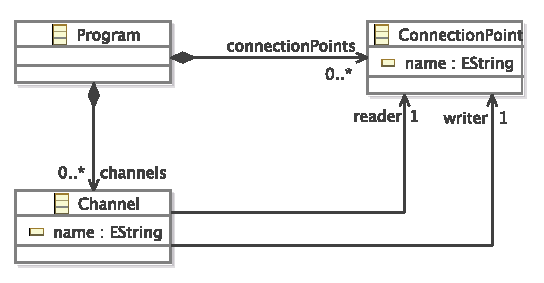
\includegraphics[width=6cm]{6.Evaluation/images/user_driven/po_before.pdf}
	}
	\subfigure[Part of the evolved metamodel.]
	{
	    \label{fig:po_evolved_mm}
	    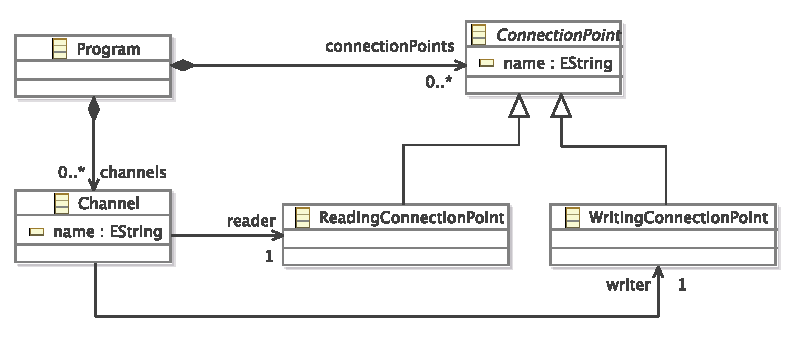
\includegraphics[width=8cm]{6.Evaluation/images/user_driven/po_after.pdf}
	}
	\caption{Process-oriented metamodel evolution.}
\label{fig:po_mms}
\end{figure}

Following the metamodel changes, a new version of the graphical editor was generated automatically from the metamodel using GMF. An annotation on the writing connection points metaclass was used to indicate to GMF that black ellipses were to be used to represent writing connection points in the graphical notation.

\subsubsection{Testing}
Testing the new version of the graphical editor highlighted the need for model migration. Attempting to load existing models, such as the one shown in Figure~\ref{fig:po_original_editor}, caused an error because \texttt{Co\-nn\-ec\-ti\-onP\-oi\-nt} was now an abstract class. Any model specifying at least one connection point no longer conformed to the metamodel. Model migration was performed to re-establish conformance and to allow the models to be loaded. 

To test the graphical editor, six models had been constructed by Sampson. Following the metamodel changes described above, three of the models could no longer be loaded and required migration. Model migration could have been specified using a model migration tool, but this seemed like overkill because only three models needed to be migrated. Instead, a user-driven co-evolution approach was used.

The remainder of this section describes the way in which model migration was performed for the changes to the process-oriented metamodel outlined above.
The sequel describes the way in which migration was performed during the development of the process-oriented metamodel, without dedicated structures for performing user-driven co-evolution. Section~\ref{subsec:user-driven_co-evolution_with_dedicated_structures} describes the way in which migration could have been performed using two of the structures presented in Chapter~\ref{Implementation}. The section concludes by comparing the two approaches.

\subsection{User-Driven Co-Evolution with EMF}
During the development of the process-oriented metamodel, no structures for performing user-driven co-evolution were available. Instead, migration was performed using only those tools available in the MDE development environment, EMF, as described below.

Migration with EMF involved identifying and fixing conformance errors, as shown in Figure~\ref{fig:emf_process}. EMF reports conformance problems when a model is loaded. For the process-oriented metamodel, loading a model involved opening the model with the graphical model editor. For the model shown in Figure~\ref{fig:po_original_editor}, the conformance problems shown in the bottom pane of Figure~\ref{fig:po_original_xmi} were reported by EMF. Because EMF cannot be used to load non-conformant models, EMF provides no further assistance in migrating the models. 

\begin{figure}[htbp]
	\centering
		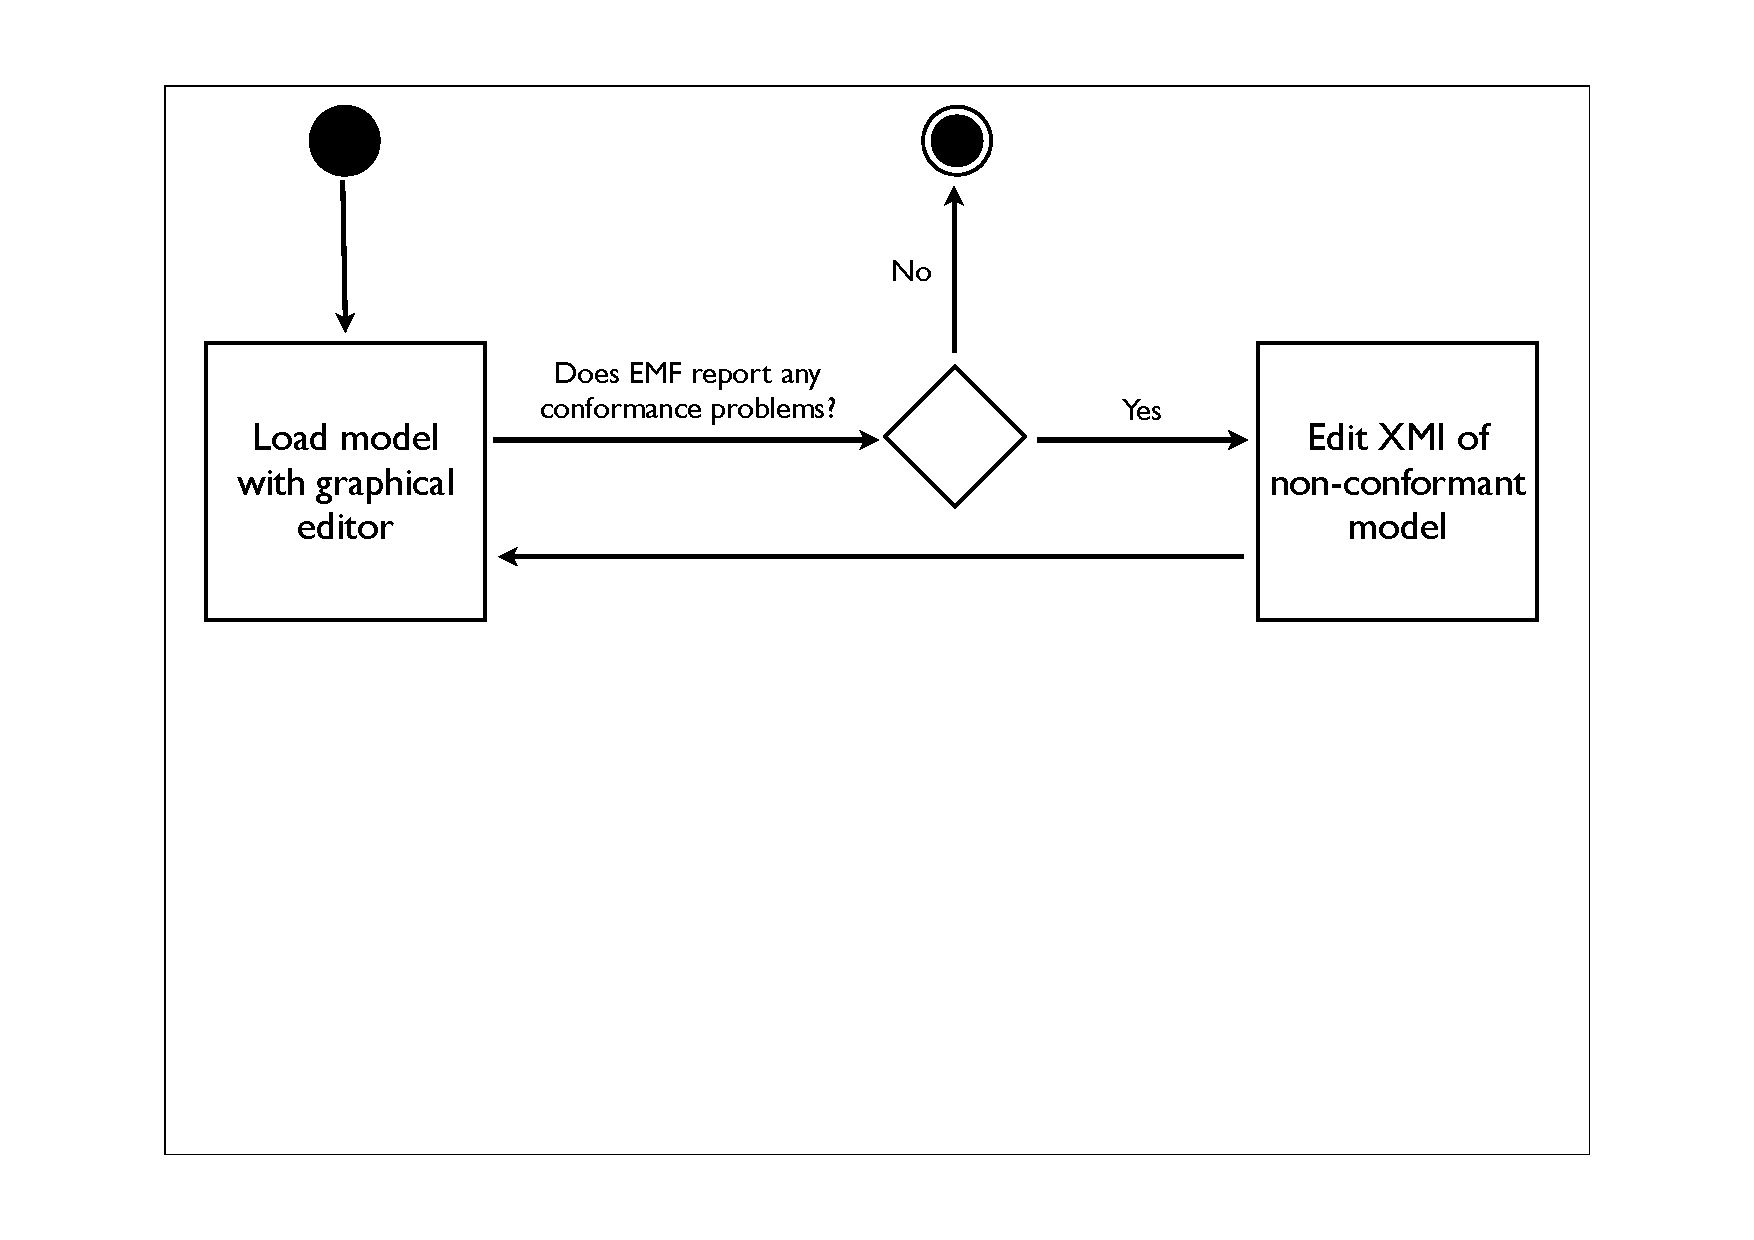
\includegraphics[width=13.5cm]{6.Evaluation/images/user_driven/emf_process.pdf}
	\caption{User-driven co-evolution with EMF}
	\label{fig:emf_process}
\end{figure}

% However, because EMF uses a multipass XMI parser, not all types of conformance problems are reported at once and, consequently, successful migration might require several iterations of the migration activities, as shown by the loops in Figure~\ref{fig:emf_process}.

Model migration proceeded manually, and involved fixing conformance problems by editing the storage representation (XMI) of the model. Figure~\ref{fig:po_original_xmi} shows the XMI for the model presented in Figure~\ref{fig:po_original_editor}. The error markers in the left-hand margin are added by EMF to indicate the conformance problems detected when the model was loaded. The conformance problems shown in Figure~\ref{fig:po_original_editor} state that ``Class `ConnectionPoint' is not found or is abstract.''

\begin{figure}[htbp]
	\centering
	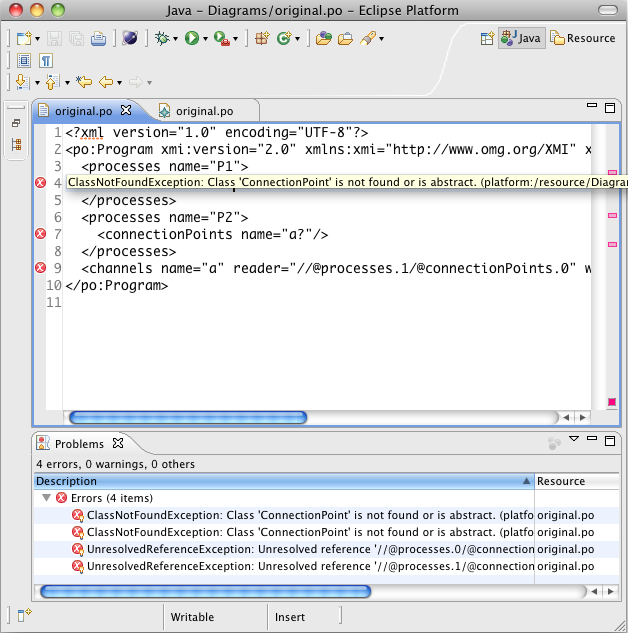
\includegraphics[width=13.5cm]{6.Evaluation/images/user_driven/po_original_xmi.png}
	\caption{XMI prior to migration}
	\label{fig:po_original_xmi}
\end{figure}

Fixing the conformance problems involved changing the type of the connection point objects to either a reading or a writing connection point. A reading (writing) connection point was used when the connection point was referenced via the \texttt{reader} (\texttt{writer}) reference of \texttt{Channel}. The reconciled XMI is shown in Figure~\ref{fig:po_migrated_xmi}. On lines X-Y, the connection point model elements have been changed to include \texttt{xmi:type} attributes, which specify whether the connection point should instantiate \texttt{ReadingConnectionPoint} or \texttt{WritingConnectionPoint}.

\begin{figure}[htbp]
	\centering
	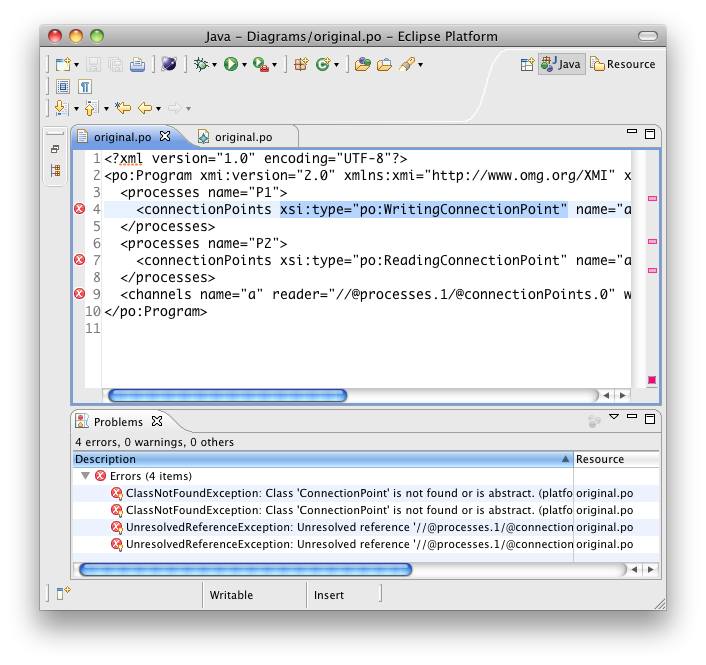
\includegraphics[width=13.5cm]{6.Evaluation/images/user_driven/po_migrated_xmi.png}
	\caption{XMI after migration}
	\label{fig:po_migrated_xmi}
\end{figure}

Reconciling the conformance problems by editing the XMI required considerable knowledge of the XMI specification. For example, the \texttt{xmi:type} attribute is used to specify the type of the connection point model elements. In fact, it must be included for those model elements, as discussed in the sidebar. However, for some of the model elements in Figure~\ref{fig:po_migrated_xmi} such as the channels, the \texttt{xmi:type} attribute need not be specified. The \texttt{xmi:type} attribute is discussed further in the sidebar.

\begin{framed}
\textbf{The \texttt{xmi:type} attribute} \\
In XMI, each model element specifies a value for the \texttt{xmi:type} attribute to indicate the metaclass that the model element instantiates. For example, the model element definition on line X of Figure~\ref{fig:po_migrated_xmi} instantiates the metaclass named \texttt{Process}. To reduce the size of models on disk, the XMI specification allows implementations to omit type information when it can be inferred. For example, line Y of Figure~\ref{fig:po_migrated_xmi} defines a model element that is contained in the \texttt{channels} reference of a \texttt{Process}. Because the \texttt{channels} reference can contain only one type of model element (\texttt{Channel}s), the \texttt{xmi:type} attribute can be omitted. Instead, the type information is inferred from the metamodel.
\end{framed}

% For every instance of \texttt{Ch\-an\-n\-el} that referenced a \texttt{Co\-nn\-ec\-ti\-o\-nPo\-i\-nt}, the following message was produced: ``Unresolved reference `\texttt{<ID>}' '' where \texttt{<ID>} was the identifier of the referenced \texttt{Co\-nn\-ec\-ti\-o\-nPo\-i\-nt}.

% Notice that conformance problem markers are still present in Figure~\ref{fig:po_original_editor}

% Iterative problem reporting might be good - perhaps it could be used to show "likely" root cause problems first, and problems less likely to be a root cause later?

Some mistakes were made when the models were migrated by manually editing the XMI. For example, in one model a \texttt{Co\-nn\-ec\-ti\-onPo\-in\-t} was replaced with the wrong subtype (a \texttt{Re\-ad\-i\-ngCo\-nn\-ec\-ti\-o\-nPo\-i\-nt} rather than a \texttt{Wr\-i\-ti\-ngCo\-nn\-ec\-ti\-o\-nPo\-i\-nt}). The mistake occurred because XMI identifies model elements using randomly generated strings. For example, consider the XMI shown in Listing~\ref{lst:po_xmi_mistake}. The two connection points on lines X and Y have very similar XMI IDs (\texttt{\_MeFREC8sEd69s-McmXQlqQ} and \texttt{\_M7EvEC8sEd69s-McmXQlqQ}), which arguably makes it more difficult to determine, from line Z, which connection point is the a reader and which is the writer. A similar situation arose -- in a model with more channels and connection points -- during the development of the process-oriented metamodel, and a mistake was made when migrating the model.


\begin{lstlisting}[caption=XMI containing elements with similar IDs, label=lst:po_xmi_mistake, language=XML]
<?xml version="1.0" encoding="UTF-8"?>
<po:Program xmi:version="2.0" xmlns:xmi="http://www.omg.org/XMI" xmlns:xsi="http://www.w3.org/2001/XMLSchema-instance" xmlns:po="po">
  <processes>
    <connectionPoints xmi:id="_MeFREC8sEd69s-McmXQlqQ" xsi:type="po:ReadingConnectionPoint" name="in"/>
    <connectionPoints xmi:id="_M7EvEC8sEd69s-McmXQlqQ" xsi:type="po:WritingConnectionPoint" name="out"/>
  </processes>
  <channels name="c" reader="_MeFREC8sEd69s-McmXQlqQ" writer="_M7EvEC8sEd69s-McmXQlqQ"/>
</po:Program>
\end{lstlisting}


As demonstrated above, migration using only the tools provided by EMF was an iterative process, and mistakes were made. Switching between the graphical model editor to determine conformance problems and a text editor to fix the problems might reduce developer productivity. Similar, fixing arguably avoidable mistakes made during migration might also reduce developer productivity. The sequel demonstrates that, using the dedicated structures described in Chapter~\ref{Implementation}, developers need not switch between editors to identify and reconcile conformance problems. In addition, the sequel suggests how the mistake described above might be avoided by using a textual modelling notation that has been optimised for humans, such as HUTN (an implementation of which was presented in Chapter~\ref{Implementation}).


\subsection{User-Driven Co-Evolution with Dedicated Structures}
\label{subsec:user-driven_co-evolution_with_dedicated_structures}

Chapter~\ref{Implementation} describes two structures that can be used to perform user-driven co-evolution. Here, the functionality of the two structures, a metamodel-independent syntax and a textual modelling notation, is summarised. Subsequently, an approach that uses the metamodel-independent syntax and the textual modelling notation for migrating the models from the process-oriented example is presented.

The metamodel-independent syntax presented in Section~\ref{sec:mmi_syntax} allows non-conformant models to be loaded, and for the conformance of models to be checked against any metamodel. The textual modelling notation presented in Section~\ref{sec:notation} is built atop the metamodel-independent syntax and provides an alternative to XMI for editing models with a textual representation. Together, the two structures can be used for performing user-driven co-evolution using the approach shown in Figure~\ref{fig:hutn_process}.

\begin{figure}[htbp]
	\centering
		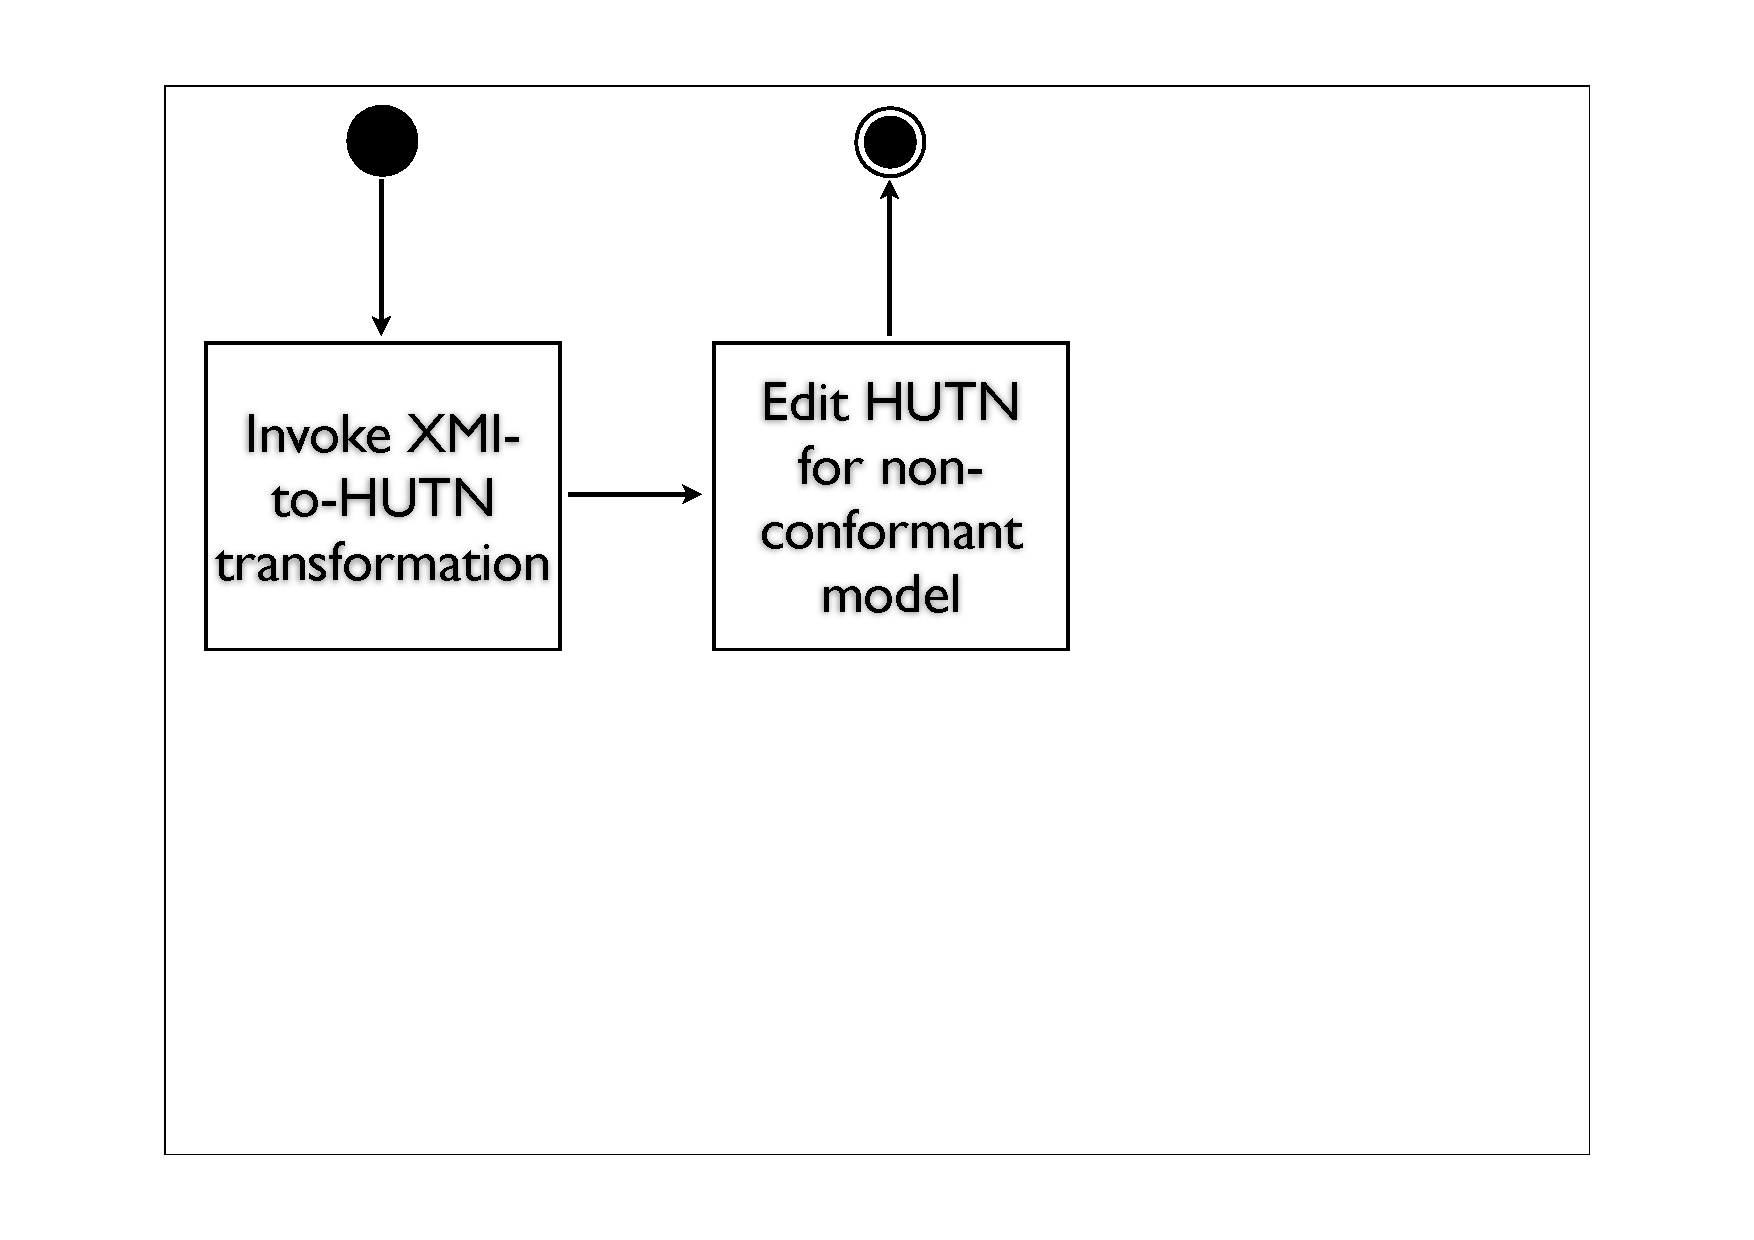
\includegraphics[width=13.5cm]{6.Evaluation/images/user_driven/hutn_process.pdf}
	\caption{User-driven co-evolution with dedicated structures}
	\label{fig:hutn_process}
\end{figure}

The way in which the approach shown in Figure~\ref{fig:hutn_process} might have been used for performing user-driven co-evolution for the process-oriented metamodel is now demonstrated. First, HUTN for the model is automatically generated after the user selects a model and clicks the ``Generate HUTN'' menu item. For the model shown in Figures~\ref{fig:po_original_xmi} and~\ref{fig:po_original_editor}, the HUTN shown in Figure~\ref{fig:po_hutn} was generated. Because the HUTN implementation presented in Chapter~\ref{Implementation} is built atop the metamodel-independent syntax, conformance is checked automatically and problems are presented in the left-hand margin of the HUTN editor. 

\begin{figure}[htbp]
  \centering
  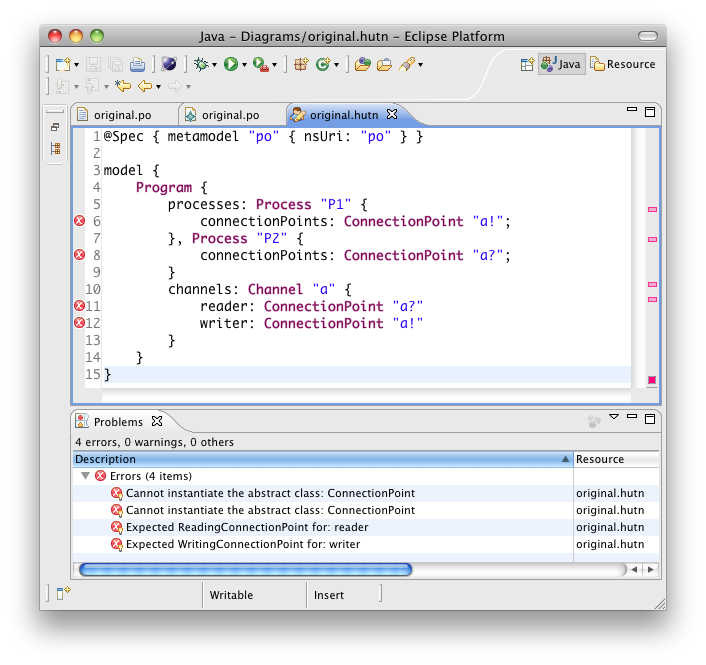
\includegraphics[width=13.5cm]{6.Evaluation/images/user_driven/po_hutn.png}
  \caption{HUTN source prior to migration}
  \label{fig:po_hutn}
\end{figure}

Conformance problems are reconciled manually by the user, who edits the HUTN source. The HUTN editor automatically checks conformance while the user edits the HUTN source. Figure~\ref{fig:po_hutn_partial} shows the HUTN editor when migration is partially complete. Some of the conformance problems have been reconciled, and the error-markers are no longer displayed in the left-hand margin.

\begin{figure}[htbp]
  \centering
  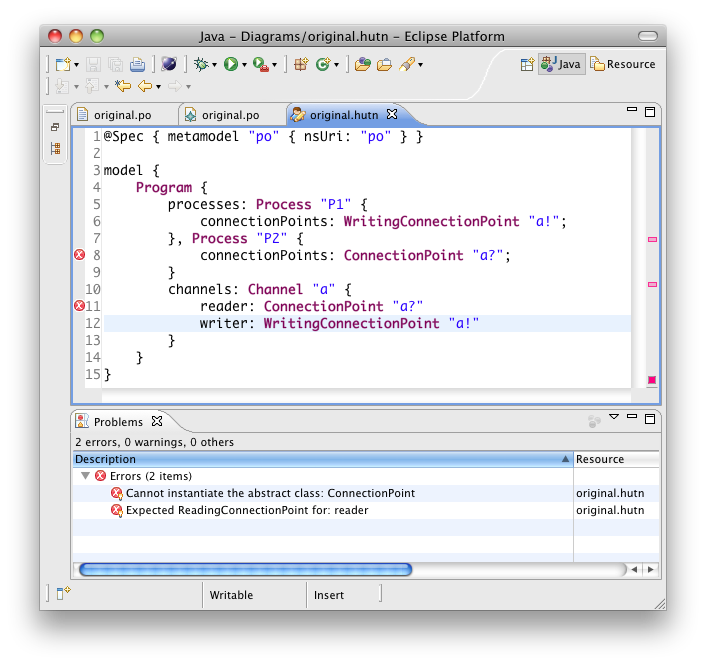
\includegraphics[width=13.5cm]{6.Evaluation/images/user_driven/po_hutn_partial.png}
  \caption{HUTN source part way through migration}
  \label{fig:po_hutn_partial}
\end{figure}

Unlike XMI, HUTN is optimised for use by humans \cite{hutn}. For the HUTN shown in Figure~\ref{fig:po_hutn}, reconciling the conformance problems involved change the type of connection points. In HUTN, every model element declaration specifies a type. Model elements of type \texttt{ConnectionPoint} were changed to instantiate \texttt{ReadingConnectionPoint} or \texttt{WritingConnectionPoint}. When all of the conformance problems are fixed and the HUTN source is saved, HUTN automatically regenerates the XMI for the model. The model can then be loaded with, for  example, a graphical editor, as was the case for the process-oriented models.


\subsection{Comparison}
\label{subsec:user_driven_example_comparison}
The two approaches to user-driven co-evolution demonstrated in this section are now compared. The comparison highlights the advantages of using the dedicated structures for user-driven co-evolution proposed in this thesis, rather than performing user-driven co-evolution without dedicated structures. The two approaches differ in the way in which conformance problems are reported, ...


The conformance reporting tool presented in Section~\ref{sec:mmi_syntax} can report more types of conformance problem at once than the model loading mechanism of EMF because the former uses a multi-pass parser, while the latter uses a single-pass parser. For the metamodel changes shown in Figure~\ref{fig:po_evolved_mm}, both the conformance reporting tool and the EMF loading mechanism reported that the evolved metamodel did not permit instantiation of the abstract class \texttt{Co\-nn\-ec\-ti\-o\-nPo\-i\-nt}. Another type of conformance problem -- the type of \texttt{Ch\-an\-n\-el\#re\-ad\-er} (\texttt{Ch\-an\-n\-el\#wr\-it\-er}) must be a \texttt{Re\-ad\-i\-ngCo\-nn\-ec\-ti\-o\-nPo\-i\-nt} (\texttt{Wr\-i\-ti\-ngCo\-nn\-ec\-ti\-o\-nPo\-i\-nt}) -- was reported by the conformance reporting tool when it was first invoked and reported by the loading mechanism of EMF only when it was invoked after the first category of conformance problem was fixed.

Secondly, the implementation of HUTN described in Section~\ref{sec:notation} uses a background incremental compiler that checks both the syntax and conformance of the HUTN source code. On the other hand, EMF checks conformance only when a model is loaded (by the graphical model editor, in this case). Saving XMI to disk does not cause EMF to check its conformance.

Thirdly, migration involved changing the types of some model elements. In XMI, when the type of a model element can be inferred from the context in which it is instantiated, type information is omitted. This reduces the size of the model on disk, but can be problematic for model migration. For example, in the original process-oriented metamodel (Figure~\ref{fig:po_original_mm}) any model element contained in the \texttt{Pr\-og\-r\-am\#co\-nn\-ec\-ti\-onPo\-in\-ts} reference must be an instance of \texttt{Co\-nn\-ec\-ti\-onPo\-in\-t}, and type information can be omitted from the XMI. When the process-oriented metamodel evolved to allow \texttt{Re\-ad\-i\-ngCo\-nn\-ec\-ti\-o\-nPo\-i\-nt} and \texttt{Wr\-i\-ti\-ngCo\-nn\-ec\-ti\-o\-nPo\-i\-nt}s to be contained in the \texttt{Pr\-og\-r\-am\#co\-nn\-ec\-ti\-onPo\-in\-ts}, type information must be added. To add type information to XMI, the person performing migration must know the correct syntax, for example: \texttt{xsi:type="po.Re\-ad\-i\-ngCo\-nn\-ec\-ti\-onPo\-i\-nt"}. By contrast, the type of every model element is declared explicitly in HUTN. As such, every HUTN document contains examples of how type information should be specified. Hence, changing the type of a model element in HUTN is arguably more straightforward than in XMI.

Finally, migration involved understanding which \texttt{Ch\-an\-n\-el}s referenced which \texttt{Co\-nn\-ec\-ti\-onPo\-in\-t}s.  By default, EMF uses universally unique identifiers (UUIDs) such as \texttt{\_M7EvEC8sEd69s-McmXQlqQ} -- or URI fragments (document-specific relative paths) such as \texttt{\\@co\-nn\-ec\-ti\-onPo\-in\-ts.0} -- to identify model elements. By contrast, the implementation of HUTN described in Chapter~\ref{Implementation}, uses the value of a model element's name feature (where one is defined) to identify model elements. For example, in Figure~\ref{fig:po_hutn} the \texttt{Ch\-an\-n\-el} on line 14 refers to \texttt{Co\-nn\-ec\-ti\-onPo\-in\-t}s by name (lines 16 and 17). Hence, referencing model elements in HUTN is arguably more straightforward than in XMI.


\subsection{Summary}
\label{subsec:user_driven_example_summary}
This section has demonstrated existing and new user-driven co-evolution processes using an example taken from a real-world project in which a metamodel was developed incrementally. Comparison of the two processes highlights several benefits of the proposed process, which used tools described in Chapter~\ref{Implementation}.


Further research is required to more rigorously assess the differences between the two user-driven co-evolution processes discussed in this section. In particular, the textual modelling notation used in the proposed process, HUTN, purports to be human-usable \cite{hutn}, but no usability studies have compared HUTN with other model representations, such as XMI. The implementation of tools for performing user-driven co-evolution, described in Chapter~\ref{Implementation}, enable further comparisons, but a thorough investigation of their usability is beyond the scope of this thesis.

This section has used two of the tools described in Chapter~\ref{Implementation} to demonstrate a user-driven co-evolution process that provides a conformance report and allows the editing of non-conformant models in a textual modelling notation. The benefits of the proposed process have been highlighted by comparison to an existing user-driven co-evolution process using a co-evolution example, taken from a project that used user-driven co-evolution.